\documentclass{tutorial}
\usepackage{tikz, tkz-berge, multirow}
\usetikzlibrary{arrows,%
                petri,%
                topaths}%
\def\checkmark{\tikz\fill[scale=0.4](0,.35) -- (.25,0) -- (1,.7) -- (.25,.15) -- cycle;} 
\begin{document}
\newif\ifsolns

%%%%%%%%%%%%%%%%%%%%%%%%%
% UNCOMMENT BELOW TO TURN ON SOLNS %
%%%%%%%%%%%%%%%%%%%%%%%%%
%\solnstrue

\title{EE241 Spring 2015: Tutorial \#5}
\date{Friday, Feb. 13, 2015}
\maketitle


\begin{prob} Fill in the following table with $0$, $1$, or $\infty$ solutions possible (multiple answer possible in one cell), or write DNA for ``does not apply''.
\begin{center}\def\arraystretch{1.75} \begin{tabular}{|ccc||c|c|c|}
\hline
System & RREF & Pivots & $m<n$ & $m=n$ & $m>n$\\
\hline
\hline
\multicolumn{1}{|l|}{\multirow{4}{*}{$A\vec{x} = \vec{b}$}}
  & \multirow{2}{1in}{$A$ has row(s) of all $0$ in RREF}
    & \multicolumn{1}{|l||}{$[A,b]$ has a pivot in the last column}
      & \multicolumn{3}{c|}{\ifsolns $0$ solutions \fi} \\ \cline{3-6}
\multicolumn{1}{|l|}{}
  & & \multicolumn{1}{|l||}{$[A,b]$ has no pivots in the last column}
      & \ifsolns $\infty$ \fi & \ifsolns $\infty$ \fi & \ifsolns $1$ or $\infty$ \fi \\ \cline{2-6}
\multicolumn{1}{|l|}{}
  & \multirow{2}{1in}{$A$ no row(s) of all $0$ in RREF}
    & \multicolumn{1}{|l||}{$[A,b]$ has a pivot in the last column}
      & \multicolumn{2}{c|}{\ifsolns $0$ solutions \fi} & \multicolumn{1}{c|}{\multirow{2}{*}{\ifsolns DNA \fi}}\\ \cline{3-5}
\multicolumn{1}{|l|}{}
  & & \multicolumn{1}{|l||}{$[A,b]$ has no pivots in the last column}
      & \ifsolns $\infty$ \fi & \ifsolns $1$ \fi & \\ \hline
\multicolumn{1}{|l|}{\multirow{2}{*}{$A\vec{x} = \vec{0}$}}
  & \multicolumn{2}{l||}{$A$ has row(s) of all $0$ in RREF}
      & \ifsolns $\infty$ \fi & \ifsolns $\infty$ \fi & \ifsolns $1$ or $\infty$ \fi \\ \cline{2-6}
\multicolumn{1}{|l|}{}
  & \multicolumn{2}{l||}{$A$ no row(s) of all $0$ in RREF}
      & \ifsolns \infty \fi & \ifsolns 1 \fi & \ifsolns DNA \fi \\ \hline
\end{tabular} \end{center}
\end{prob}

\begin{prob}[Fitting] The first three \emph{physicists' Hermite polynomials} are the following
\begin{align*}
  H_0(x) &= 1, \\
  H_1(x) &= 2x, \\
  H_2(x) &= 4x^2-2.
\end{align*}
Find a linear combination of these polynomials such that the resulting function passes through $(0,0)$ $(1,0)$, and the first derivative at $x=1$ is $-1$.
\end{prob} \ifsolns \begin{proof}
First, let $f(x) = b_0H_0(x) + b_1H_1(x) + b_2H_2(x)$. The three conditions we have are that $f(0)=0$, $f(1)=0$, and the $df/dx|_1=-1$. Consider the first derivative of $f(x)$,
\begin{align*}
  \frac{df}{dx} &= b_0 \frac{dH_0}{dx} + b_1 \frac{dH_1}{dx} + b_2 \frac{dH_2}{dx} \\
  &= b_0 \cdot 0 + b_1 \cdot 2 + b_2 \cdot (8x) \\
  & = 2b_1H_0(x) + 4b_2H_1(x)
\end{align*}
In the last line, I've rewritten the polynomial in terms of the original $H_i(x)$ to show that the derivative operation doesn't produce functions that cannot be written as a linear combination of $H_i(x)$. Now our three conditions are
\[
  \lb \begin{array}{rlcl}
    0 &= b_0 -2b_2& \hspace{0.15in} \text{from} \hspace{0.15in} & f(0)=0 \\
    0 &= b_0 + 2b_1 + 2b_2 & \hspace{0.15in} \text{from} \hspace{0.15in} & f(1)=0 \\
   -1 &= 2b_1 + 8b_2 & \hspace{0.15in} \text{from} \hspace{0.15in} & df/dx|_1=-1
  \end{array} \right.
\]
The linear system for $\vec{b} = \ls b_0, b_1, b_2 \rs$ can be solved by row reduction on
\[
  \ls A| \vec{f} \rs
  = \ls \begin{array}{rrr|r}
    1 & 0 &-2 & 0 \\
    1 & 2 & 2 & 0 \\
    0 & 2 & 8 &-1 \\
  \end{array} \rs
  \hspace{0.25in} \longrightarrow \hspace{0.25in}
  \ls \begin{array}{rrr|r}
    1 & 0 & 0 &-1/2 \\
    0 & 1 & 0 & 1/2 \\
    0 & 0 & 1 &-1/4 \\
  \end{array} \rs
\]
Thus $\vec{b} = \ls -1/2, 1/2, -1/4 \rs$ and 
\[
  \boxed{f(x) = -1/2 H_0(x) + 1/2 H_1(x) - 1/4 H_2(x) = x-x^2 .}
\]
\end{proof}\else \newpage \fi

\begin{prob}[Permutations]
Group the following permutations into even and odd,
\[
  \lb 1, 2, 4, 3 \rb \; , \;
  \lb 1, 4, 2, 3 \rb \; , \;
  \lb 4, 1, 2, 3 \rb \; , \;
  \lb 4, 1, 3, 2 \rb \; , \;
  \lb 4, 3, 1, 2 \rb \; , \;
  \lb 4, 3, 2, 1 \rb
\]
\end{prob} \ifsolns \begin{proof}
The first permutation is odd (swap $3$ and $4$) and every other permutation in the list results from one swap on the previous permutation. Thus, the groups are
\begin{align*}
  \text{even} &= \lb 1, 4, 2, 3 \rb \; , \; \lb 4, 1, 3, 2 \rb \; , \; \lb 4, 3, 2, 1 \rb \\
  \text{odd}  &= \lb 1, 2, 4, 3 \rb \; , \; \lb 4, 1, 2, 3 \rb \; , \; \lb 4, 3, 1, 2 \rb .
\end{align*}
\end{proof}\else \vspace{2in} \fi


\begin{prob}[Vector lengths]
Which is longer: a $n$-dimensional vector of $1$'s? Or a $2n$-dimensional vector of $1/2$'s?
\end{prob} \ifsolns \begin{proof}
A $n$-dimensional vector of $1$'s has length
\[ \sqrt{\sum_{i=1}^n (1)^2} = \sqrt{n} . \]
A $2n$-dimensional vector of $1/2$'s' has length
\[ \sqrt{\sum_{i=1}^{2n} (1/2)^2} = 1/2 \cdot \sqrt{2n} = \sqrt{n/2} . \]
Thus, the vector of $1$'s is longer.
\end{proof}\else \vspace{2in} \fi


\begin{prob}[Determinants] Find the determinant of the following matrix
\[
  \ls \begin{array}{ccccc}
    1&1&0&0&0\\
    1&1&1&0&0\\
    0&1&1&1&0\\
    0&0&1&1&1\\
    0&0&0&1&1
  \end{array} \rs .
\]
\end{prob} \ifsolns \begin{proof}
First, reorder the rows to get as close as possible to upper-triangular form,
\[
  \ls \begin{array}{ccccc}
    1&1&1&0&0\\
    0&1&1&1&0\\
    0&0&1&1&1\\
    0&0&0&1&1\\
    1&1&0&0&0
  \end{array} \rs .
\]
Now subtract the first row and add the third row to the fifth row to get
\[
  \ls \begin{array}{ccccc}
    1&1&1&0&0\\
    0&1&1&1&0\\
    0&0&1&1&1\\
    0&0&0&1&1\\
    0&0&0&1&1
  \end{array} \rs .
\]
Now subtract the fourth row from the fifth to get
\[
  \ls \begin{array}{ccccc}
    1&1&1&0&0\\
    0&1&1&1&0\\
    0&0&1&1&1\\
    0&0&0&1&1\\
    0&0&0&0&0
  \end{array} \rs .
\]
Since there is a row of $0$'s, the determinant itself is also $0$.
\end{proof}\else \newpage \fi

\begin{prob}
The graph below represents the following process: You are steering a ship probabilistically. Your first mate flips two fair coins every half-an-hour. If he gets two heads, you turn the ship around. Otherwise, you turn the ship $90^{\circ}$ ``starboard" (right). This graph contains no self-loops, i.e.: a ``stay'' is not a valid move.
\begin{center} 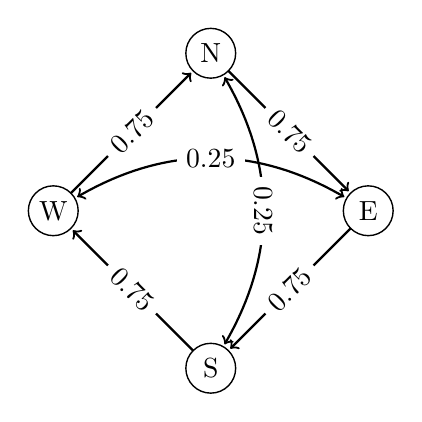
\begin{tikzpicture}[scale=1,transform shape]
  \Vertex[x= 2,y= 4] N
  \Vertex[x= 4,y= 2] E 
  \Vertex[x= 2,y= 0] S 
  \Vertex[x= 0,y= 2] W
  \tikzstyle{LabelStyle}=[fill=white,sloped]
  \tikzstyle{EdgeStyle}=[post]
  \Edge[label=$0.75$](N)(E)
  \Edge[label=$0.75$](E)(S)
  \Edge[label=$0.75$](S)(W)
  \Edge[label=$0.75$](W)(N)
  \tikzstyle{EdgeStyle}=[pre and post, bend left]
  \Edge[label=$0.25$](N)(S)
  \tikzstyle{EdgeStyle}=[pre and post, bend right]
  \Edge[label=$0.25$](E)(W)
\end{tikzpicture} \end{center}
\begin{enumerate}[label=(\alph*)]
\item What is the matrix $M$ representing this Markov process? This matrix should transform the vector $\vec{p} = \ls p_N, p_E, p_S, p_W \rs$ to new probabilities $\vec{p}'$ according to the rules of the coin flips. (To check your answer, you can apply the matrix to $\vec{p} = \ls 1,0,0,0 \rs, \ls 0,1,0,0 \rs, \dots$).
\item You have no idea which direction you initially set sail in ($\vec{p}$). However, after an hour and a half, you estimate the following probabilities for your direction $\vec{p}' = \ls 9/64, 27/64, 27/64, 1/64 \rs$. Which direction did you set sail in?
\end{enumerate}
\end{prob} \ifsolns \begin{proof}
\begin{enumerate}
\item The $(i,j)$ entry of the matrix $M$ are the probability of transitioning from direction $j$ (column, ``input'') to direction $i$ (row, ``output''). Thus
\[
  M = \ls \begin{array}{rrrr}
      0 & 3/4 & 1/4 &   0 \\
      0 &   0 & 3/4 & 1/4 \\
    1/4 &   0 &   0 & 3/4 \\
    3/4 & 1/4 &   0 &   0 \\
  \end{array} \rs .
\]
\item After an hour and a half we've made $3$ transitions, so we need to calculate $M^3$. To help with our mental math, let's calculate $N^3$ instead where $N=4M$ (we won't need to worry about denominators).
\begin{align*}
  N^3 & = \ls \begin{array}{rrrr}
      0 &   3 &   1 &   0 \\
      0 &   0 &   3 &   1 \\
      1 &   0 &   0 &   3 \\
      3 &   1 &   0 &   0 \\
  \end{array} \rs \ls \begin{array}{rrrr}
      0 &   3 &   1 &   0 \\
      0 &   0 &   3 &   1 \\
      1 &   0 &   0 &   3 \\
      3 &   1 &   0 &   0 \\
  \end{array} \rs \ls \begin{array}{rrrr}
      0 &   3 &   1 &   0 \\
      0 &   0 &   3 &   1 \\
      1 &   0 &   0 &   3 \\
      3 &   1 &   0 &   0 \\
  \end{array} \rs \\
  & =  \ls \begin{array}{rrrr}
      0 &   3 &   1 &   0 \\
      0 &   0 &   3 &   1 \\
      1 &   0 &   0 &   3 \\
      3 &   1 &   0 &   0 \\
  \end{array} \rs \ls \begin{array}{rrrr}
      1 &   0 &   9 &   6 \\
      6 &   1 &   0 &   9 \\
      9 &   6 &   1 &   0 \\
      0 &   9 &   6 &   1 \\
  \end{array} \rs \\
  & =  \ls \begin{array}{rrrr}
     27 &   9 &   1 &  27 \\
     27 &  27 &   9 &   1 \\
      1 &  27 &  27 &   9 \\
      9 &   1 &  27 &  27 \\
  \end{array} \rs
\end{align*}
Now $M^3 = N^3/4^3$ so
\[
  M^3 = \ls \begin{array}{rrrr}
     27/64 &   9/64 &   1/64 &  27/64 \\
     27/64 &  27/64 &   9/64 &   1/64 \\
      1/64 &  27/64 &  27/64 &   9/64 \\
      9/64 &   1/64 &  27/64 &  27/64 \\
  \end{array} \rs
\]
Our original direction and our new estimated direction are related by $\vec{p}' = M^3 \vec{p}$. The natural thing to do would be to find $(M^3)^{-1}$ and solve $\vec{p} = (M^3)^{-1} \vec{p}'$. However, we can use a special fact about $\vec{p}$ to simplify our work. Since $\vec{p}$ represents only one of four directions, we can test the four associated vectors to check which of them solves $\vec{p}' = M^3 \vec{p}$. The four directions are
\[
  \vec{p} \in \lb 
    \ls \begin{array}{r} 1 \\ 0 \\ 0 \\ 0 \end{array} \rs, 
    \ls \begin{array}{r} 0 \\ 1 \\ 0 \\ 0 \end{array} \rs, 
    \ls \begin{array}{r} 0 \\ 0 \\ 1 \\ 0 \end{array} \rs, 
    \ls \begin{array}{r} 0 \\ 0 \\ 0 \\ 1 \end{array} \rs 
  \rb .
\]
Each of these vectos, in order, returns the first, second, third, and fourth column of $M^3$ when we calculate $M^3 \vec{p}$. Thus, we just need to find \emph{which} column of $M^3$ is identical to $\vec{p}'$. This happens to be the second column, and so we conclude that we must have initially been heading East.
\end{enumerate}
\end{proof}\else \vspace{4in} \fi


\end{document}